\section{Cara insert SQLite}
	\subsection{Definisi}
		\begin{enumerate}
			\item SQLite adalah sistem manajemen basis data relasional yang terkandung dalam pustaka pemrograman C. Tidak seperti banyak sistem manajemen basis data lainnya, SQLite bukan mesin basis data client-server. Semuanya, dicetak dalam program terakhir.
			\item SQLite adalah ACID-compliant dan mengimplementasikan sebagian besar standar SQL, menggunakan sintaks SQL dinamis dan yang tidak dapat menjamin integritas domain..
		\end{enumerate}
	\subsection{Sejarah}
		\begin{enumerate}
			\item D. Richard Hipp mendesain SQLite pada musim semi tahun 2000 ketika bekerja untuk General Dynamics dalam kontrak dengan Angkatan Laut Amerika Serikat. Hipp merancang perangkat lunak yang digunakan pada kapal perusak rudal, yang semula menggunakan HP-UX dengan database back-end IBM Informix. SQLite dimulai sebagai ekstensi Tcl.
			\item Tujuan desain dari SQLite adalah untuk memungkinkan program untuk beroperasi tanpa menginstal sistem manajemen basis data atau membutuhkan administrator basis data. Hipp berdasarkan sintaks dan semantik pada PostgreSQL 6.5. Pada bulan Agustus 2000, versi 1.0 dari SQLite dirilis, dengan penyimpanan berdasarkan gdbm (GNU Database Manager). SQLite 2.0 menggantikan gdbm dengan implementasi B-tree khusus, menambahkan kemampuan transaksi. SQLite 3.0, sebagian didanai oleh America Online, menambahkan internasionalisasi, pengetikan manifes, dan peningkatan besar lainnya.
			\item Pada tahun 2011 Hipp mengumumkan rencana untuk menambahkan antarmuka NoSQL (mengelola dokumen yang dinyatakan dalam JSON) ke database SQLite dan mengembangkan UnQLite, database berorientasi dokumen yang dapat disematkan. UnQLite dirilis sebagai database independen.
		\end{enumerate}
	\subsection{Desain}
		\begin{enumerate}
			\item Tidak seperti sistem manajemen basis data client-server, mesin SQLite tidak memiliki proses mandiri yang digunakan aplikasi untuk berkomunikasi. Sebaliknya, pustaka SQLite terhubung dan dengan demikian menjadi bagian integral dari program aplikasi. Menautkan dapat berupa statis atau dinamis. Program aplikasi menggunakan fungsi SQLite melalui panggilan fungsi sederhana, yang mengurangi latensi dalam akses database: panggilan fungsi dalam satu proses lebih efisien daripada komunikasi antar-proses. SQLite menyimpan seluruh basis data (definisi, tabel, indeks, dan datanya sendiri) sebagai file lintas platform tunggal pada mesin host. Ini mengimplementasikan desain sederhana ini dengan mengunci seluruh file database saat menulis. Operasi baca SQLite dapat multitasked, meskipun menulis hanya dapat dilakukan secara berurutan.
			\item Karena desainnya tanpa server, aplikasi SQLite memerlukan lebih sedikit konfigurasi daripada database client-server. SQLite disebut nol-conf karena tidak memerlukan manajemen layanan (seperti skrip startup) atau kontrol akses berdasarkan GRANT dan kata sandi. Kontrol akses ditangani dengan cara izin sistem file yang diberikan ke file database itu sendiri. Database dalam sistem client-server menggunakan hak akses file sistem yang memberikan akses ke file database hanya ke proses daemon.
			\item Implikasi lain dari desain tanpa server adalah bahwa beberapa proses mungkin tidak dapat menulis ke file database. Dalam basis data berbasis server, beberapa penulis akan terhubung ke daemon yang sama, yang mampu menangani kunci secara internal. Di sisi lain, SQLite harus bergantung pada kunci sistem file. Ini memiliki sedikit pengetahuan tentang proses lain yang mengakses database pada saat yang bersamaan. Oleh karena itu, SQLite bukan pilihan yang lebih disukai untuk penyebaran intensif. Namun, untuk pertanyaan sederhana dengan sedikit konkurensi, keuntungan kinerja SQLite dari menghindari overhead yang meneruskan datanya ke proses lain.
			\item SQLite menggunakan PostgreSQL sebagai platform referensi. Apa yang akan dilakukan PostgreSQL digunakan untuk memahami standar SQL. Salah satu ketidakberesan utama adalah bahwa, dengan pengecualian kunci primer, SQLite tidak memaksakan jenis pemeriksaan; jenis nilai bersifat dinamis dan tidak dibatasi oleh skema (meskipun skema akan memicu konversi saat menyimpan, jika konversi semacam itu berpotensi reversibel). SQLite berusaha mengikuti Aturan Postel.
		\end{enumerate}
		
		\subsection{Syntax Perintah Insert}
\begin{verbatim}

INSERT INTO nama_tabel [(kolom1, kolom2, kolom3, … kolomn)]
VALUES (nilai1, nilai2, nilai3,… nilaiN);
Kolom1, kolom2, kolom3 merupakan nama kolom yang ada didalam tabel sqlite yang akan kamu tambahkan data kedalam masing masing kolom tersebut.

INSERT INTO nama_tabel VALUES (nilai1, nilai2, nilai3,… nilaiN);
Contoh Perintah Insert Di SQLite


INSERT INTO siswa (id, nama, umur, alamat)
VALUES (1, 'Firdan Ardiansyah',27,'JL. KH. Atim II');
INSERT INTO siswa (id, nama, umur, alamat)
VALUES (2, 'Muhammad Ammar',25,'BTN. Palaton');
INSERT INTO siswa (id, nama, umur, alamat)
VALUES (3, 'Bilal Ardiansyah',23,'BTN. Depag');
INSERT INTO siswa (id, nama, umur, alamat)
VALUES (4, 'Rafi Syabani',25,'BTN. Sumur Buang');

INSERT INTO siswa VALUES (5, 'Muhammad Bintang',23,'Pandeglang'); 
Melihat Data Didalam Tabel Siswa
\end{verbatim}


	\subsection{Melihat Data}
		\begin{verbatim}
SELECT * FROM siswa;
		\end{verbatim}
		
	\begin{figure}[ht]
		\centerline{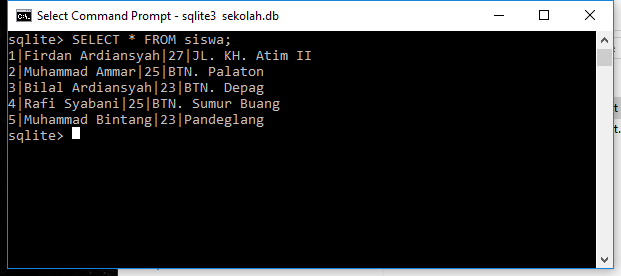
\includegraphics[width=1\textwidth]{figures/Sql.png}}
		\caption{Hasilnya}
		\label{Sql}
	\end{figure}
	Gambar \ref{Sql} Hasil gambar.
	
	\subsection{Fiture}
		\begin{enumerate}
			\item SQLite mengimplementasikan sebagian besar standar SQL-92 untuk SQL tetapi tidak memiliki beberapa fitur. Misalnya, beberapa menyediakan pemicu, dan tidak dapat menulis ke tampilan (tetapi menyediakan pemicu INSTEAD OF yang menyediakan fungsi ini). Meskipun menyediakan query kompleks, masih memiliki fungsi ALTER TABLE terbatas, karena tidak dapat memodifikasi atau menghapus kolom.
			\item SQLite menggunakan sistem tipe yang tidak biasa untuk DBMS yang kompatibel dengan SQL: alih-alih menetapkan jenis ke kolom seperti pada kebanyakan sistem basis data SQL, mereka ditetapkan ke nilai individual: dalam bahasa yang diketik secara dinamis. Selain itu, itu lemah diketik dalam beberapa cara yang sama bahwa Perl adalah: satu dapat memasukkan string ke dalam kolom integer (meskipun SQLite akan mencoba untuk mengubah string ke integer pertama, jika jenis kolom yang diinginkan adalah bilangan bulat). Ini menambah fleksibilitas ke kolom, terutama ketika terikat ke bahasa scripting yang diketik secara dinamis. Namun, teknik ini tidak portabel untuk produk SQL lainnya. Kritik umum adalah bahwa sistem tipe SQLite tidak memiliki mekanisme integritas data yang disediakan oleh kolom-kolom yang diketik secara statis dalam produk lain. Situs web SQLite menggambarkan mode afinitas yang ketat, tetapi fitur ini belum ditambahkan. Namun, itu dapat diimplementasikan dengan pembatasan semacam itu. Tabel biasanya menyertakan kolom index rowid tersembunyi yang memberikan akses lebih cepat. Jika database termasuk kolom Integer Primary Key, SQLite biasanya akan mengoptimalkannya dengan memperlakukannya sebagai alias untuk rowid, menyebabkan kontennya disimpan sebagai integer 64-bit yang diketik-ketat dan mengubah perilakunya menjadi agak seperti penambahan otomatis kolom. Versi masa depan dari SQLite mungkin termasuk perintah untuk mengintrospeksi apakah sebuah kolom memiliki perilaku seperti itu dari rowid untuk membedakan kolom ini dari Kunci Primer Integer yang tidak terkunci secara otomatis.
			\item SQLite dengan fungsi Unicode penuh adalah opsional.
			\item Beberapa proses komputer atau utas dapat mengakses basis data yang sama secara bersamaan. Beberapa akses dapat dibaca secara paralel. Akses hanya dapat digunakan jika ada. Jika tidak, akses tulis gagal dengan kode kesalahan (atau dapat dicoba kembali secara otomatis sampai batas waktu dapat dikonfigurasi untuk kedaluwarsa). Akses data ini akan berubah ketika berhadapan dengan tabel sementara. Pembatasan ini dilonggarkan dalam versi 3,7 dari kompilasi write-ahead (WAL) diaktifkan untuk memungkinkan membaca dan pencurian simultan. SQLite versi 3.7.4 pertama kali melihat modul FTS4 tambahan (pencarian teks lengkap), menampilkan perbaikan dalam modul FTS3 yang lebih lama. FTS4 memungkinkan pengguna untuk melakukan teks lengkap pada dokumen yang mirip dengan bagaimana mesin pencari mencari halaman web. Versi 3.8.2 Tambah untuk membuat tabel tanpa rowid, yang dapat memberikan ruang dan peningkatan kinerja. Penguatan tabel umum ditambahkan ke SQLite di versi 3.8.3.
		\end{enumerate}
	\subsection{Perkembangan dan Distribusi}
		\begin{enumerate}
			\item Kode SQLite di-host dengan Fossil, sistem kontrol versi terdistribusi yang dibangun di database SQLite.
			\item Program baris perintah yang berdiri sendiri disediakan dalam distribusi SQLite. Ini dapat digunakan untuk membuat database, menentukan tabel, menyisipkan dan mengubah baris, menjalankan kueri dan mengelola file database SQLite. Ini juga berfungsi sebagai contoh untuk menulis aplikasi yang menggunakan pustaka SQLite.
			\item SQLite menggunakan pengujian regresi otomatis sebelum setiap rilis. Lebih dari 2 juta tes dijalankan sebagai bagian dari verifikasi rilis. Dimulai dengan rilis 10 Agustus 2009 dari SQLite 3.6.17, rilis SQLite memiliki cakupan cabang cakupan 100%, salah satu komponen cakupan kode. Tes dan tes menggunakan domain publik dan kepemilikan parsial.
		\end{enumerate}
	\subsection{SQLite Serverless}
		\begin{enumerate}
			\item Sebagian besar mesin database SQL diimplementasikan sebagai proses server terpisah. Program yang ingin mengakses database berkomunikasi dengan server menggunakan beberapa jenis komunikasi interprocess (biasanya TCP / IP) untuk mengirim permintaan ke server dan menerima hasilnya kembali. SQLite tidak berfungsi dengan cara ini. Dengan SQLite, proses yang ingin mengakses database membaca dan menulis langsung dari file database pada disk. Tidak ada proses server menengah.
			\item Ada kelebihan dan kekurangan menjadi serverless. Keuntungan utama adalah tidak ada proses server terpisah untuk menginstal, mengkonfigurasi, mengkonfigurasi, menginisialisasi, mengelola, dan memecahkan masalah. Ini adalah salah satu alasan mengapa SQLite adalah mesin database "konfigurasi-nol". Program yang menggunakan SQLite tidak memerlukan dukungan administratif untuk menyiapkan mesin basis data sebelum dijalankan. Setiap program yang dapat mengakses disk dapat menggunakan database SQLite.
			\item Di sisi lain, mesin database yang menggunakan server dapat memberikan perlindungan yang lebih baik dari bug di aplikasi klien - pointer liar pada klien tidak dapat merusak memori di server. Dan karena server adalah proses persisten tunggal, ia mampu mengontrol akses basis data dengan lebih presisi, memungkinkan penguncian yang lebih baik dan konkurensi yang lebih baik.
			\item Sebagian besar mesin klien / server database berbasis SQL. Dari mereka tanpa server, SQLite adalah satu-satunya yang diketahui dari penulis ini yang memungkinkan beberapa aplikasi untuk mengakses database yang sama pada saat yang bersamaan.
			\item Biasanya, RDBMS seperti MySQL, PostgreSQL, dll, membutuhkan proses server terpisah untuk beroperasi. Aplikasi yang ingin mengakses server database menggunakan protokol TCP / IP untuk mengirim dan menerima permintaan. Ini disebut arsitektur client / server.
		\end{enumerate}
	\subsection{Neo Serverless vs Classic Serverless}
		\begin{enumerate}
			\item Baru-baru ini, orang mulai menggunakan kata serverless berarti sesuatu yang sangat berbeda dari makna yang dimaksudkan dalam dokumen ini. 
			\item Berikut dua definisi yang mungkin tanpa server:
			\item Classic Serverless: Mesin database berjalan dalam proses, thread, dan ruang alamat yang sama dengan aplikasi. Tidak ada pesan yang lewat atau aktivitas jaringan.
			\item Neo-Serverless: Mesin database berjalan di ruang nama aplikasi terpisah, mungkin pada mesin yang terpisah, tetapi database disediakan sebagai layanan turn-key oleh penyedia hosting, yang tidak memerlukan manajemen atau administrasi dari pemilik aplikasi, dan sangat mudah digunakan bahwa pengembang dapat mengasumsikan database sebagai serverless bahkan jika server benar-benar menggunakan di bawah selimut.
			\item SQLite adalah contoh mesin database tanpa server klasik. Dengan SQLite, tidak ada proses, thread, mesin, atau mekanisme lain (selain OS host komputer dan sistem file) untuk membantu menyediakan layanan atau implementasi database. Sama sekali tidak ada server.
			\item Microsoft Azure Cosmo DB dan Amazon S3 adalah contoh dari database neo-serverless. Database ini diimplementasikan oleh proses server yang berjalan secara terpisah di cloud. Tetapi server dikelola dan dikelola oleh ISP, bukan oleh pengembang aplikasi. Pengembang aplikasi hanya menggunakan layanan ini. Pengembang tidak harus menyediakan, mengkonfigurasi, atau mengelola instance server basis data, karena semua pekerjaan ditangani secara otomatis oleh penyedia layanan. Server database memang ada, mereka hanya tersembunyi dari para pengembang.
			\item Penting untuk memahami dua definisi yang berbeda ini untuk serverless. Ketika sebuah database mengklaim sebagai serverless, pastikan untuk mengetahui apakah itu berarti serverless klasik atau neo-serverless.
		\end{enumerate}

		\subsection{Mandiri}
		\begin{enumerate}
		\item SQLite adalah alat mandiri yang memerlukan dukungan minimal dari sistem operasi atau pustaka eksternal. Ini membuat SQLite dapat digunakan di lingkungan apa pun terutama di perangkat yang tertanam seperti iPhone, ponsel Android, konsol game, pemutar media genggam, dll.
		\item SQLite dikembangkan menggunakan ANSI-C. Kode sumber tersedia sebagai sqlite3.c besar dan file header-nya sqlite3.h. Jika Anda ingin mengembangkan aplikasi yang menggunakan SQLite, Anda hanya perlu memasukkan file-file ini ke dalam proyek Anda dan kompilasi dengan kode Anda.
		\end{enumerate}
		
		\subsection{Kesimpulan}
			\begin{enumerate}
				\item SQLite adalah pusat dalam pemrosesan yang mengimplementasikan server di database SQL sendiri, tanpa server, nol - konfigurasii, transakssional. Kode untuk SQLite ada di domain publik dan dengan demikian bebas digunakan untuk tujuan apa pun, komersial atau pribadi. SQLite adalah database yang paling banyak digunakan di dunia dengan aplikasi lebih dari yang dapat kita hitung, termasuk beberapa proyek profil tinggi.
				\item SQLite adalah mesin basis data SQL tertanam. Tidak seperti kebanyakan database SQL lainnya, SQLite tidak memiliki proses server terpisah. SQLite membaca dan menulis langsung ke file disk biasa. Database SQL lengkap dengan banyak tabel, indeks, pemicu, dan tampilan, terdapat dalam satu file disk. Format file database adalah cross-platform - Anda dapat dengan bebas menyalin database antara sistem 32-bit dan 64-bit atau antara arsitektur big-endian dan little-endian. Fitur-fitur ini menjadikan SQLite pilihan populer sebagai Format File Aplikasi. Pikirkan SQLite bukan sebagai pengganti Oracle tetapi tidak fopen ().
				\item SQLite adalah pustaka yang ringkas. Dengan semua fitur diaktifkan, ukuran pustaka bisa kurang dari 500KiB, tergantung pada platform target dan pengaturan optimasi kompilator. (Kode 64-bit lebih besar, dan beberapa optimisasi kompilator seperti inlining fungsi agresif dan dekomposisi loop dapat menyebabkan kode objek menjadi jauh lebih besar.) Ada tradeoff antara penggunaan memori dan kecepatan. SQLite umumnya berjalan lebih cepat, semakin banyak memori yang Anda berikan. Namun demikian, kinerja biasanya cukup baik bahkan dalam lingkungan memori yang rendah. Tergantung pada bagaimana itu digunakan, SQLite bisa lebih cepat daripada filesystem langsung I atau O.
				\item SQLite sangat hati-hati diuji sebelum rilis masing-masing dan memiliki reputasi sebagai sangat dapat diandalkan. Sebagian besar kode sumber SQLite spesifik untuk pengujian dan verifikasi. Sebuah rangkaian uji otomatis menjalankan jutaan dan jutaan kasus uji coba yang melibatkan ratusan juta pernyataan SQL individual dan mencapai cakupan cakupan 100%. SQLite merespon dengan anggun untuk kegagalan alokasi memori dan disk I / O kesalahan. Transaksi adalah ACID bahkan jika terganggu oleh sistem crash atau gangguan listrik. Semua ini diverifikasi oleh tes otomatis menggunakan alat uji khusus yang mensimulasikan kegagalan sistem. Tentu saja, bahkan dengan semua tes ini, masih ada bug. Tapi tidak seperti beberapa proyek serupa (terutama pesaing komersial) SQLite terbuka dan jujur ​​tentang semua bug dan memberikan daftar bug dan kronologi menit-demi-menit dari perubahan kode.
				\item Basis kode SQLite didukung oleh tim pengembangan internasional yang bekerja pada SQLite penuh waktu. Pengembang terus memperluas kemampuan SQLite dan meningkatkan keandalan dan kinerja mereka sambil mempertahankan kompatibilitas mundur dengan spesifikasi antarmuka yang dipublikasikan, sintaks SQL, dan format file database. Kode sumbernya benar-benar gratis bagi siapa saja yang menginginkannya, tetapi dukungan profesional juga tersedia.
				\item Proyek SQLite dimulai pada 2000-05-09. Masa depan selalu tidak dapat diprediksi, tetapi maksud dari pengembang adalah untuk mendukung SQLite sepanjang tahun 2050. Keputusan desain dibuat dengan mengingat tujuan tersebut.
				\item Kami pengembang berharap bahwa Anda menemukan SQLite berguna dan kami meminta Anda untuk menggunakannya dengan baik: untuk membuat produk cantik dan indah yang cepat, andal, dan mudah digunakan. Carilah pengampunan untuk diri sendiri saat Anda memaafkan orang lain. Dan sama seperti Anda telah menerima SQLite gratis, jadi berikan juga gratis, bayar utang ke depan.
			\end{enumerate}
			
\cite{owens2010sqlite}
\cite{newman2004sqlite}
\cite{kreibich2010using}
\cite{kang2013x}
\cite{jeon2012recovery}
\cite{lee2012creating}

\subsection{insert sqlite language}
\begin{enumerate}
\itemSisipan Bahasa Query Sqlite
Pernyataan INSERT hadir dalam tiga bentuk dasar.
1. INSERT INTO table VALUES (...);
Bentuk pertama (dengan kata kunci "VALUES") membuat satu atau lebih baris baru dalam tabel yang ada. Jika daftar nama kolom setelah nama tabel dihilangkan, maka jumlah nilai yang dimasukkan ke setiap baris harus sama dengan jumlah kolom dalam tabel. Dalam hal ini, hasil evaluasi ekspresi paling kiri dari setiap istilah daftar VALUES dimasukkan ke dalam kolom paling kiri dari setiap baris baru, dan seterusnya untuk setiap ekspresi berikutnya. Jika daftar kolom-nama ditentukan, maka jumlah nilai dalam setiap jangka waktu daftar VALUE harus sesuai dengan jumlah kolom yang ditentukan. Setiap kolom bernama dari baris baru diisi dengan hasil mengevaluasi ekspresi VALUES yang sesuai. Kolom tabel yang tidak muncul dalam daftar kolom diisi dengan nilai kolom default (ditetapkan sebagai bagian dari pernyataan CREATE TABLE), atau dengan NULL jika tidak ada nilai default yang ditentukan.
2. INSERT INTO table SELECT ...;
Bentuk kedua dari pernyataan INSERT berisi pernyataan SELECT bukannya klausa VALUES. Entri baru dimasukkan ke dalam tabel untuk setiap baris data yang dikembalikan dengan mengeksekusi pernyataan SELECT. Jika daftar kolom ditentukan, jumlah kolom dalam hasil SELECT harus sama dengan jumlah item dalam daftar-kolom. Jika tidak, jika tidak ada daftar kolom yang ditentukan, jumlah kolom dalam hasil SELECT harus sama dengan jumlah kolom dalam tabel. Setiap pernyataan SELECT, termasuk pernyataan gabungan SELECT dan SELECT dengan klausa ORDER BY dan / atau LIMIT, dapat digunakan dalam pernyataan INSERT dari formulir ini.
3. INSERT INTO table DEFAULT VALUES;
Bentuk ketiga dari pernyataan INSERT adalah dengan NILAI DEFAULT. Pernyataan INSERT ... DEFAULT VALUES menyisipkan satu baris baru ke dalam tabel bernama. Setiap kolom dari baris baru diisi dengan nilai default-nya, atau dengan NULL jika tidak ada nilai default yang ditetapkan sebagai bagian dari definisi kolom dalam pernyataan CREATE TABLE.
\end{enumerate}
			
			
